\documentclass[11pt]{article}

% ==== PACKAGES ==== %
% \usepackage{fullpage}
\usepackage{amsmath,amssymb,amsthm}
\usepackage{epic}
\usepackage{eepic}
\usepackage{hyperref}
\usepackage{listings}
\usepackage{float}
\usepackage{graphicx}
\usepackage{subcaption}
\usepackage{fancyhdr}
\usepackage{color}
\usepackage{bbm}
\usepackage[letterpaper, margin=1in]{geometry}

% ==== MARGINS ==== %
% \pagestyle{empty}
% \setlength{\oddsidemargin}{0in}
% \setlength{\textwidth}{6.8in}
% \setlength{\textheight}{9.5in}

\pagestyle{fancy}
\fancyhf{}
\rhead{ASEN 5044}
\lhead{Homework 7}
\rfoot{Page \thepage}

\newtheorem*{solution*}{Solution}
\newtheorem{lemma}{Lemma}[section]
\newtheorem{theorem}[lemma]{Theorem}
\newtheorem{claim}[lemma]{Claim}
\newtheorem{definition}[lemma]{Definition}
\newtheorem{corollary}[lemma]{Corollary}
\lstset{moredelim=[is][\bfseries]{[*}{*]}}

% ==== DOCUMENT PROPER ==== %
\begin{document}

\thispagestyle{empty}

% --- Header Box --- %
\newlength{\boxlength}\setlength{\boxlength}{\textwidth}
\addtolength{\boxlength}{-4mm}

\begin{center}\framebox{\parbox{\boxlength}{\bf
      Statistical Estimation \hfill Homework 7\\
      ASEN 5044 Fall 2018 \hfill Due Date: November 8, 2018\\
      Name: Andrew Kramer \hfill PhD Student
}}
\end{center}

\section*{Problem 1}

Consider an aircraft moving in a plane with constant speed (the magnitude of the velocity vector) and turning with a constant angular rate. Such a model is often used by air traffic control tracking algorithms to describe aircraft executing coordinated turns. Given 2D inertial position variables $\xi(t)$, east position, and $\eta(t)$, north position. The equations of motion are 
\begin{align*}
	\ddot{\xi} &= -\Omega\dot{\eta} \\
	\ddot{\eta} &= \Omega\dot{\xi}
\end{align*}
where $\Omega$ is the constant angular rate, such that $\Omega > 0$ implies a counterclockwise turn. Using the state representation $x(t)=[\xi,\dot{\xi},\eta,\dot{\eta}]^T$, it can be shown that 
\begin{equation*}
	e^{A\Delta t} = \begin{bmatrix} 1 & \frac{\sin(\Omega\Delta t)}{\Omega} & 0 & -\frac{1-\cos(\Omega\Delta t)}{\Omega} \\ 0 & \cos(\Omega\Delta t) & 0 & -\sin(\Omega\Delta t) \\ 0 & \frac{1-\cos(\Omega\Delta t)}{\Omega} & 1 & \frac{\sin(\Omega\Delta t)}{\Omega} \\ 0 & \sin(\Omega\Delta t) & 0 & \cos(\Omega\Delta t) \end{bmatrix}
\end{equation*}
Where $A$ is the CT LTI state matrix for the system.

\subsection*{part (a)}
Find $A$ ignoring measurements $y$ and process noise for now. What is the DT LTI model for this system (also ignoring process noise)?

\subparagraph*{}
The $A$ matrix for the continuous time system is:
\begin{equation*}
	A = \begin{bmatrix} 0 & 1 & 0 & 0 \\
						0 & 0 & 0 & -\Omega \\
						0 & 0 & 0 & 1 \\
						0 & \Omega & 0 & 0 \end{bmatrix}
\end{equation*}
Because there is no control input and no process noise, the discrete time system is described $x(k)=Fx(k-1)$ where $F=\text{exp}\{A\Delta t\}$ as given in the problem statement.


\subsection*{part (b)}
For the following questions (i)-(ii) assume a sampling time of $\Delta t=0.5$s, $\Omega=0.045\frac{\text{rad}}{\text{s}}$, and an initial DT state uncertainty $x(0)\sim\mathcal{N}(\mu(0),P(0))$ at $k=0$. Again, disregard process noise and measuremenths for now.

\subsubsection*{part (i)}
Derive an expression for the predicted DT state mean $\mu(k)=E[x(k)]$ and state covariance $P(k)=E[(x(k)-\mu(k))(x(k)-\mu(k))^T]$ for an arbitrary number of steps $k=N$ into the future, starting from $k=0$. Be sure to express your answer in terms of $N$, $\mu(0)$, and $P(0)$ and the DT state transition matrix $F$.

\subparagraph*{}
Because there is no additive process noise, the state transition from $x(0)$ to $x(1)$ is a linear function of $x(0)$. In fact, any $x(k)$ can be expressed as a function of $x(0)$ per the following:
\begin{align*}
	x(1) &= Fx(0) \\
	x(2) &= Fx(1) = F^2x(0) \\
	x(k) &= F^kx(0)
\end{align*}
So any $x(k)$ is a linear function of the random variable $x(0)$. This means the mean $\mu(N) = F^N\mu(0)$ and $P(N) = F^NP(0)(F^N)^T$. 

\subsubsection*{part (ii)}
Assume
\begin{align*}
	\mu(0) &= [0\text{m},\ 85\cos(\pi/4)\text{m/s},\ 0\text{m},\ -85\sin(\pi/4)\text{m/s}]^T \\
	P_a(0) &= \text{diag}([10\text{m}^2,\ 2\text{(m/s)}^2,\ 10\text{m}^2,\ 2\text{(m/s)}^2])
\end{align*}
Perform a 150 step calculation of $\mu(k)$ and $P(k)$ for $k=1,2,\dots,150$ starting from these initial conditions. Plot the following in separate plots:
\begin{itemize}
	\item each state element of $\mu(k)$ versus time, along with $\pm2\sigma$ upper/lower bounds showing the uncertainty for each state at each time $k$.
	\item only the positive $2\sigma$ values versus time for each state at time $k$.
\end{itemize}
Be sure to label all axis with appropriate units and comment on the results.

\subparagraph*{}
The plots in figures \ref{x1_plots} to \ref{x4_plots} show the values of each $x$ variable bounded by $2\sigma$ an subplot a and the value for $2\sigma$ in subplot b. Note the variance for the position variables $x_1$ and $x_3$ appears to be periodic over time but the variance on the velocities $x_2$ and $x_4$ is constant.

\begin{figure}
\centering
\begin{subfigure}[b]{.45\textwidth}
	\centering
	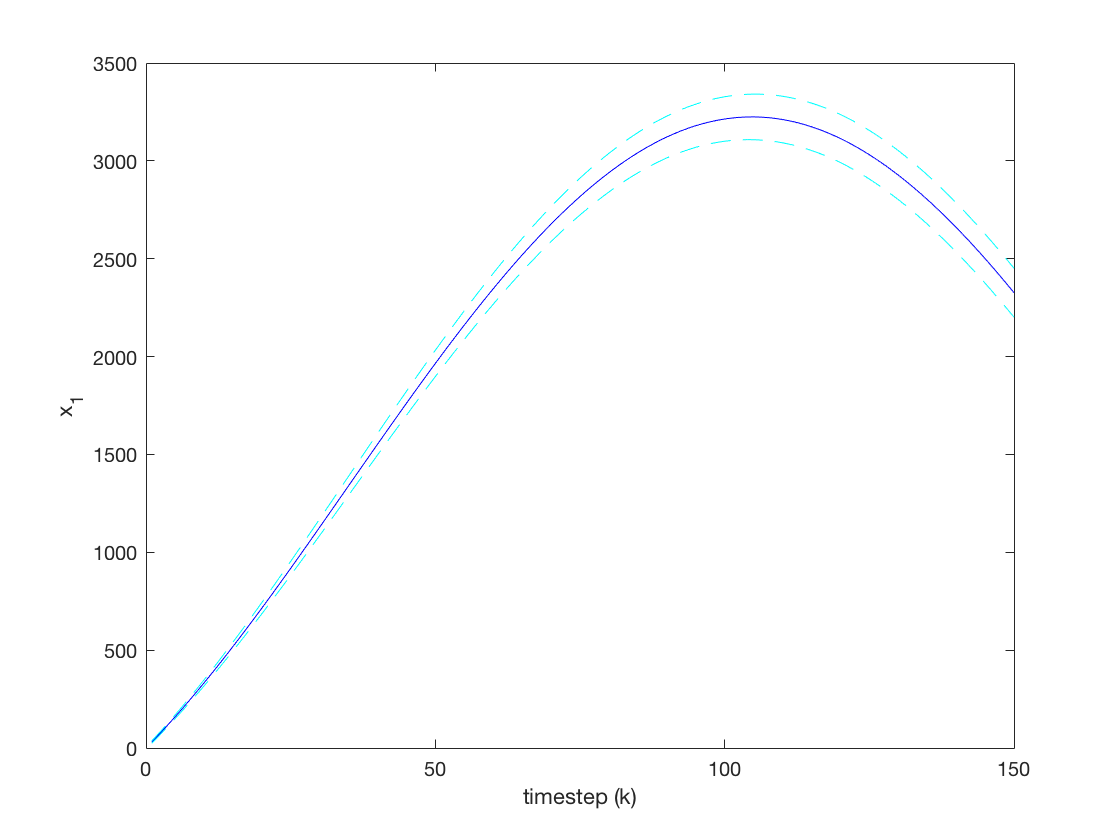
\includegraphics[width=\textwidth]{p1_plt1.png}
	\caption{$x_1$ (m) vs timestep}
	\label{x1}
\end{subfigure}
~
\begin{subfigure}[b]{.45\textwidth}
	\centering
	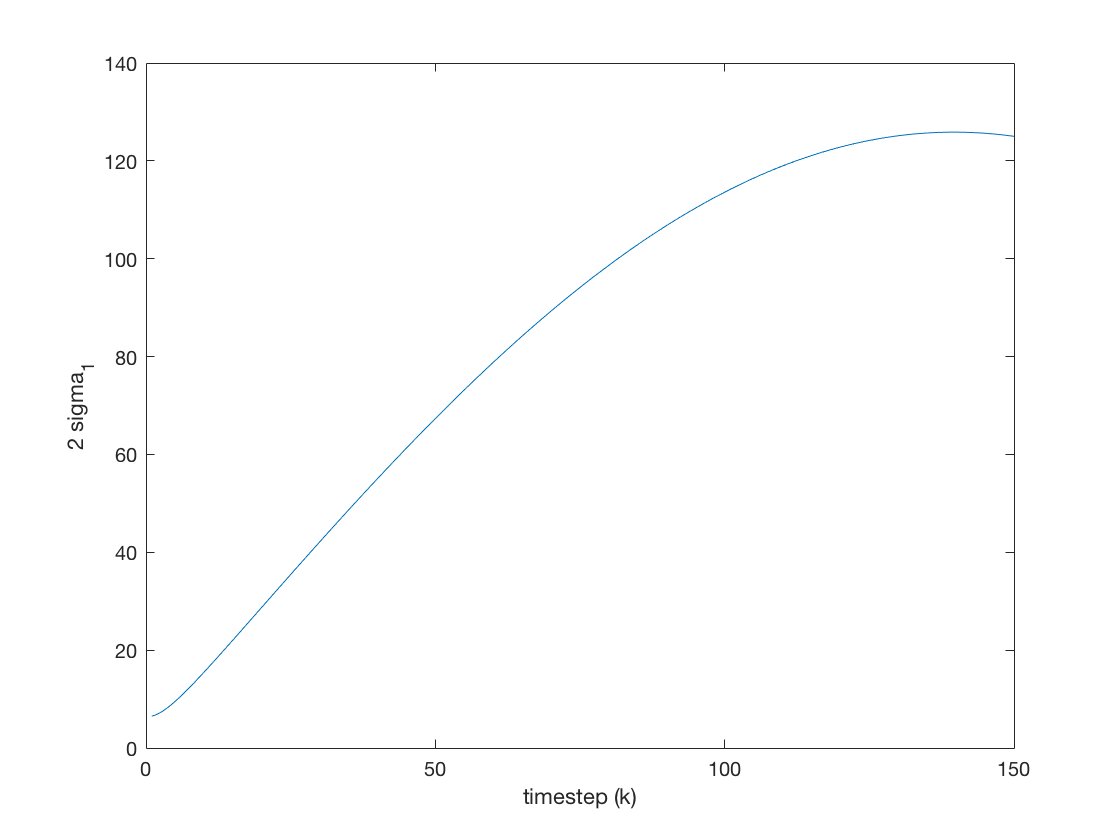
\includegraphics[width=\textwidth]{p1_plt2.png}
	\caption{$\sigma_1$ ($\text{m}^2$) vs timestep}
	\label{sigma1}
\end{subfigure}
\caption{Plots for $x_1$ and $\sigma_1$}
\label(x1_plots)
\end{figure}

\begin{figure}
\centering
\begin{subfigure}[b]{.45\textwidth}
	\centering
	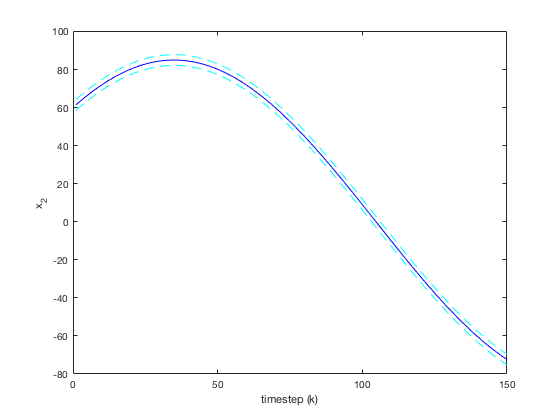
\includegraphics[width=\textwidth]{p1_plt3.png}
	\caption{$x_2$ (m/s) vs timestep}
	\label{x2}
\end{subfigure}
~
\begin{subfigure}[b]{.45\textwidth}
	\centering
	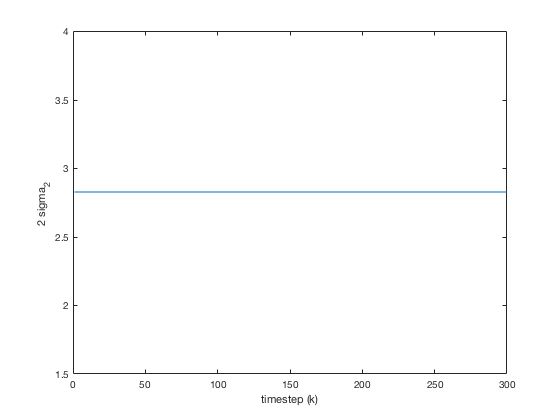
\includegraphics[width=\textwidth]{p1_plt4.png}
	\caption{$\sigma_1$ ($\text{(m/s)}^2$) vs timestep}
	\label{sigma2}
\end{subfigure}
\caption{Plots for $x_2$ and $\sigma_2$}
\label(x2_plots)
\end{figure}

\begin{figure}
\centering
\begin{subfigure}[b]{.45\textwidth}
	\centering
	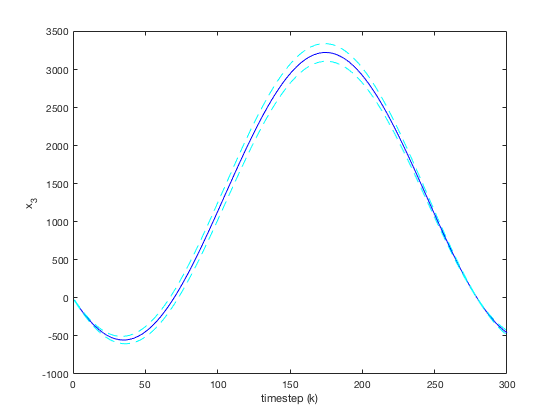
\includegraphics[width=\textwidth]{p1_plt5.png}
	\caption{$x_3$ (m) vs timestep}
	\label{x3}
\end{subfigure}
~
\begin{subfigure}[b]{.5\textwidth}
	\centering
	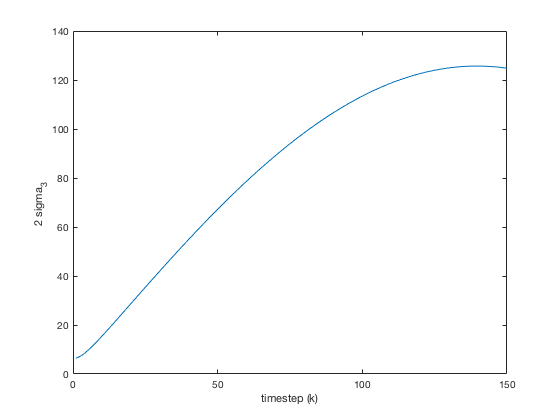
\includegraphics[width=\textwidth]{p1_plt6.png}
	\caption{$\sigma_3$ ($\text{m}^2$) vs timestep}
	\label{sigma3}
\end{subfigure}
\caption{Plots for $x_3$ and $\sigma_3$}
\label(x3_plots)
\end{figure}

\begin{figure}
\centering
\begin{subfigure}[b]{.45\textwidth}
	\centering
	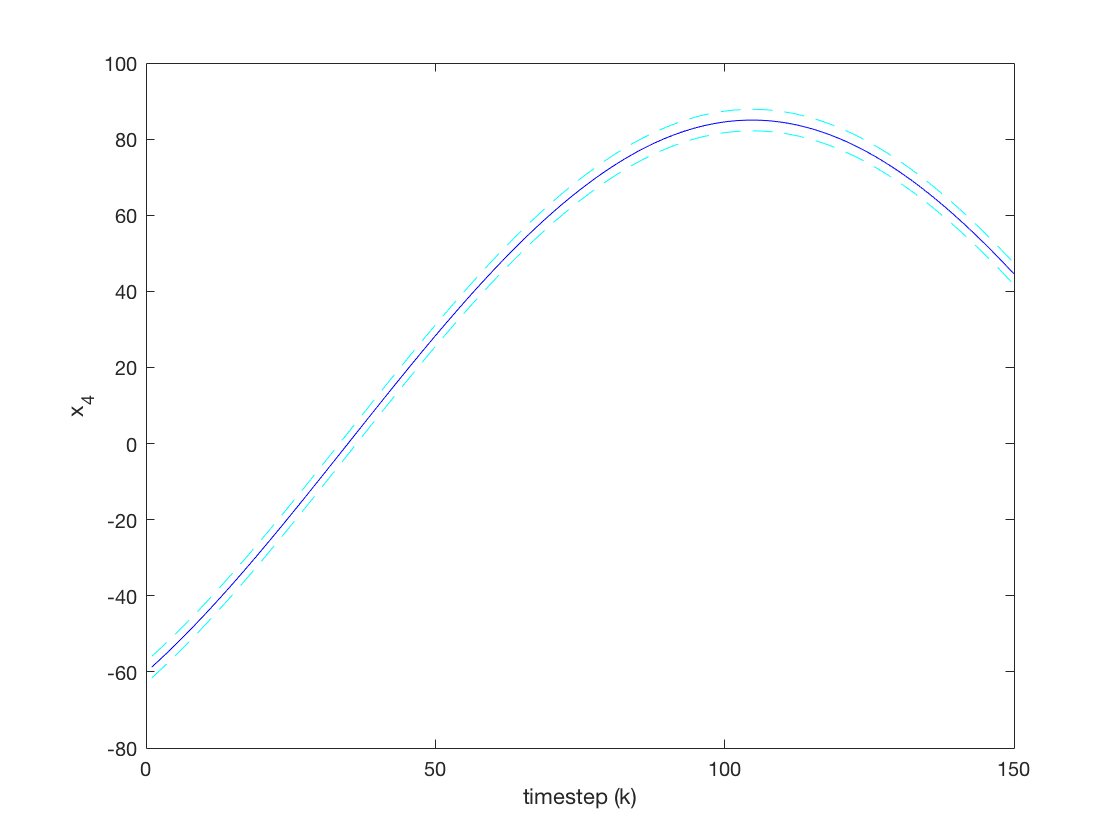
\includegraphics[width=\textwidth]{p1_plt7.png}
	\caption{$x_4$ (m/s) vs timestep}
	\label{x4}
\end{subfigure}
~
\begin{subfigure}[b]{.45\textwidth}
	\centering
	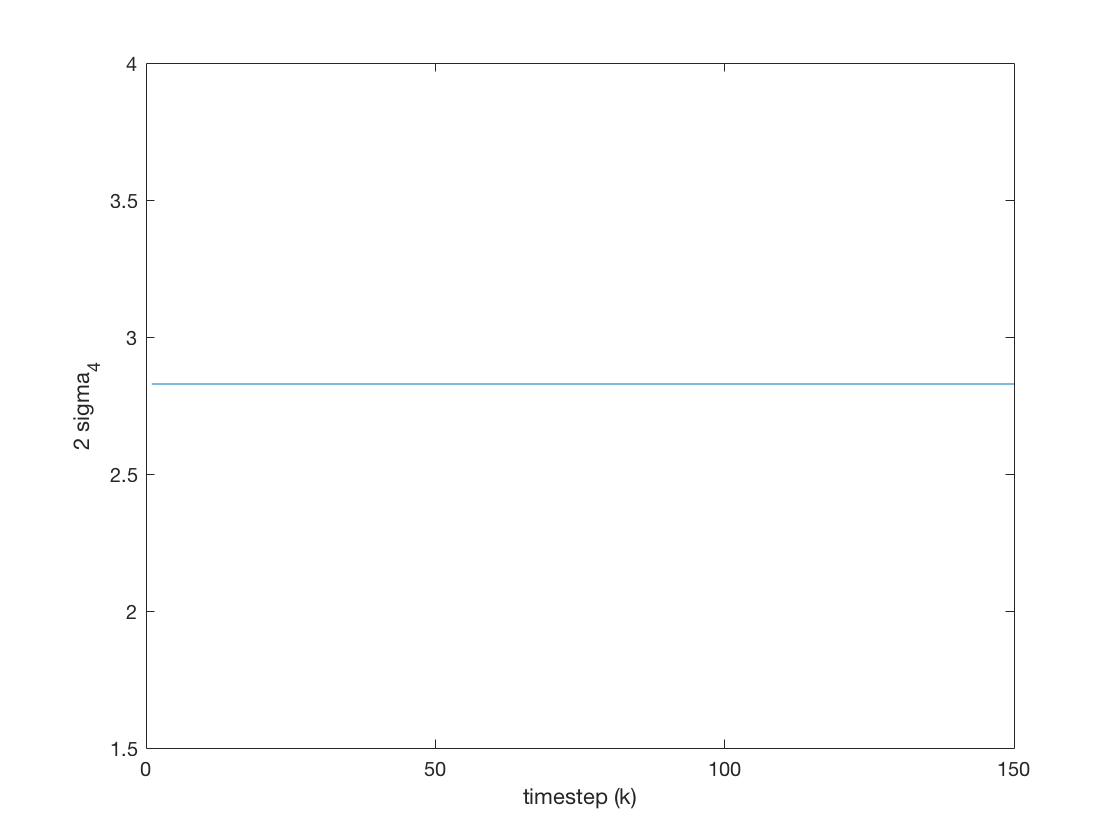
\includegraphics[width=\textwidth]{p1_plt8.png}
	\caption{$\sigma_4$ ($\text{(m/s)}^2$) vs timestep}
	\label{sigma4}
\end{subfigure}
\caption{Plots for $x_4$ and $\sigma_4$}
\label(x4_plots)
\end{figure}

\subsection*{part (c)}
Consider now computing the probability of collision for two aircraft turning independently at the same altitude at the same time, where the initial position and velocity of the aircraft are unknown. Let $x_a$ denote the state of aircraft $a$ and let $x_b$ denote the state of aircraft $b$. A collition will simply be modeled as an event where both aircraft occupy a bounded rectangular region of airspace at the same time. That is, if $r_a(k)=[\xi_a(k),\eta_a(k)]^T$ and $r_b(k)=[\xi_b(k),\eta_b(k)]^T$, a collition occurs at time $k$ whenever $r_c(k) = r_k(k)-r_b(k)$ lies inside the region $R$ defined by $\Delta\xi(k)\in[-\xi_R,\xi_R]$ and $\Delta\eta(k)\in[-\eta_R,\eta_R]$, where $\Delta\xi(k)=\xi_a(k)-\xi_b(k)$, $\Delta\eta(k)=\eta_a(k)-\eta_b(k)$, and $\xi_R$ and $\eta_R$ are known constants. At time $k=0$, suppose both aircraft states are independent and normally distributed, with $x_a(0)~\mathcal{N}(\mu_a(0),P_a(0))$ and $x_k(0)~\mathcal{N}(\mu_b(0),P_b(0))$. Also assume that $\Delta t=0.5$s, $\Omega_a=0.045$rad/s and $\Omega_b=-0.045$rad/s. Again, ignore process noise and measurements.

\subsubsection*{part (i)}
Derive the expression for the mean and covariance parameters af the pdf $p(r_c(k))$ at any time $k$, given that $r_c(k)~\mathcal{N}(\mu_{r_c}(k),P_{r_c}(k))$ (i.e. the pdf for $r_c(k)$ must be a multivariate Gaussian). Your answers should be in terms of $F_a$ and $F_b$ (the STMs for each aircraft), as well as $\mu_a(0)$, $\mu_b(0)$, and $P_a(0)$, $P_b(0)$. (\textbf{Hint:} the concept of marginalizing multivariate Gaussian pdfs will be useful here.)

\subsubsection*{part (ii)}
Use the result from part (i) to derive an integral expression for the probability of collision at any time $k$.

\subsubsection*{part (iii)}
Plot the probability of collision vs time using a simulation run of 150 seconds starting from the following initial conditions
\begin{align*}
	\mu_a(0) &= [0\text{m},\ 85\cos(\pi/4)\text{m/s},\ 0\text{m},\ -85\sin(\pi/4)\text{m/s}]^T \\
	P_a(0) &= \text{diag}([10\text{m}^2,\ 4\text{(m/s)}^2,\ 10\text{m}^2,\ 4\text{(m/s)}^2]) \\
	\mu_b(0) &= [3200\text{m},\ 85\cos(\pi/4)\text{m/s},\ 3200\text{m},\ -85\sin(\pi/4)\text{m/s}]^T \\
	P_b(0) &= \text{diag}([11\text{m}^2,\ 3.5\text{(m/s)}^2,\ 11\text{m}^2,\ 3.5\text{(m/s)}^2])
\end{align*}
and using $\xi_R=100$m, $\eta_R=100$m. Be sure to label axes with appropriate units, and comment on the results. In particular, at what time steps are the vehicles in greatest danger of colliding? Also, what happens to the probability of collision as time increases? What explains this behavior? Matlab's \texttt{mvncdf.m} command is useful here.

\end{document}
